
\chapter{Classical Braids}

We first consider the set of classical braids of \( n \) strands, \( \mathit{uB}_n \), and specifically \( B \in \mathit{uB}_n \) for \( n \in \N_{\ge 0} \). 
We define a braid \( B \) as a continuous injective function from \( n \) intervals \( I_i \subset \R \), \( i \in [n] \)  to a unit box \( [0, 1]^3 \). 
And so \( B : \bigsqcup_{i = 1}^n I_i \rightarrow [0, 1]^3 \) is a braid where the image of \( I_i \) under \( B \) is the \( i \)th strand of the braid. 
The starting positions and ending positions of the strands are linearly spaced along the bottom and top of the cube, i.e. the image of all left and right bounds of the intervals are \( \left\{ \left(\frac{i}{n + 1}, \frac{1}{2} , 0 \right) \mid i \in [n] \right\} \) and \( \left\{ \left(\frac{i}{n + 1}, \frac{1}{2} , 1 \right) \mid i \in [n] \right\} \) respectively. 

When \( B \) is restricted to a given interval \( I_i \), \( B_n |_{I_i} : I_i \rightarrow [0, 1]^3 \) is monotonically increasing in the \( z \) component. 
Intuitively, this means that any single strand cannot ``decrease in height.''

Finally, we consider the set of all \( n \)-strand braids \( \mathit{uB}_n \), and we consider these braids modulo isotopy.
Under isotopy we can deform any braid \( B \) such that the braids do not touch the side of the box \( [0, 1]^3 \). We will assume this condition is satisfied from now on. 

We finally define the set of all classical braids with any number of strands as \( \mathit{uB} \), which is the union of all \( uB_n \) for \( n \ge 0 \).

\begin{figure}[H]
    \centering
    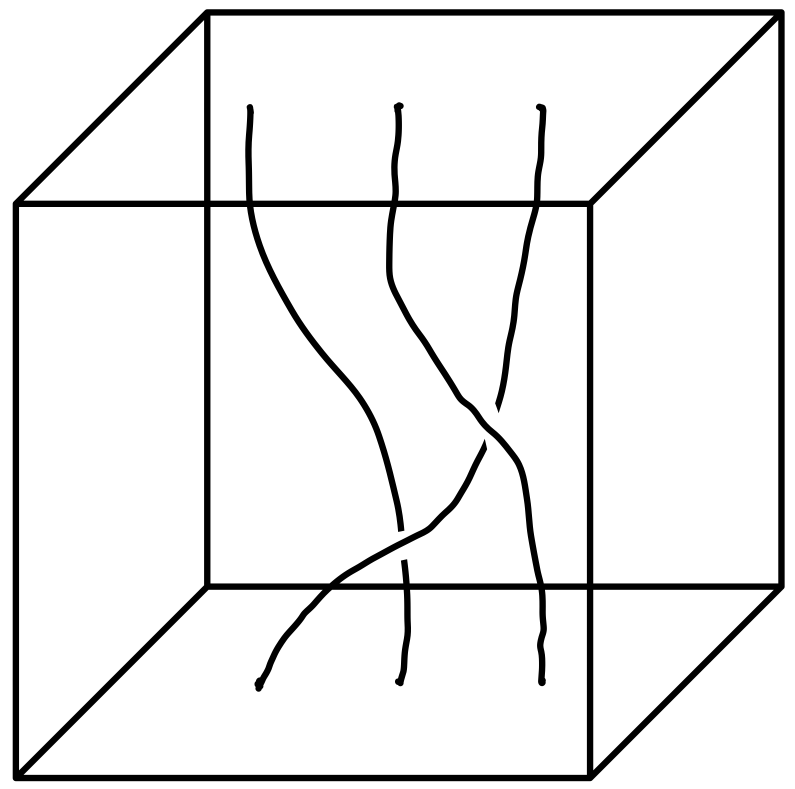
\includegraphics[width=0.4\textwidth]{classical_braids/0_classical_braid.png}
    \caption{The Image of a Braid in \( uB_3 \)}
    \label{fig:classical_braid}
\end{figure}

\section{Visualisation of Classical Braids}

We want to be able to generalise braids into the fourth dimension, as well as be able to study aspects of them such as the crossings. 
We do this by mapping the braid into different visualisations. 

The movie visualisation is used to give intuition for \( 4 \) dimensional braids, braid diagrams give intuition for crossings of a braid, and the braid group gives intuition as to the structure that crossings make. 
As they are defined and shown to be equivalent, we will use these visualisations interchangeably after this section. 

\subsection{Braids as a movie}

Let's consider a time parameter \( t \in [0, 1]\) and define a frame of \( B \) at \( t \), \( F_t(B) \) as the projection of the intersection of \( \{ (x, y, z) \in [0, 1]^3 \mid z = t \}  \) with \( Im(B) \) into the \( xy \)-plane, i.e. 
\[ F_t(B) = \{ (x, y) \in [0, 1]^2 \mid (x, y, t) \in Im(B) \} \]
In which case we can re-represent \( B \) as a movie where \( t \) is increasing from \( 0 \) to \( 1 \).  
Each one of these frames will be \( n \) points within \( [0, 1]^2 \), where each point represents a strand of the braid at that \( t \). 
% We will denote the \( i \)th strand within the frame at \( t \) for the braid \( B \) as \( F_t^i(B) \), which in all cases will be a single point in \( [0, 1]^2 \). 

\begin{figure}[H]
    \centering
    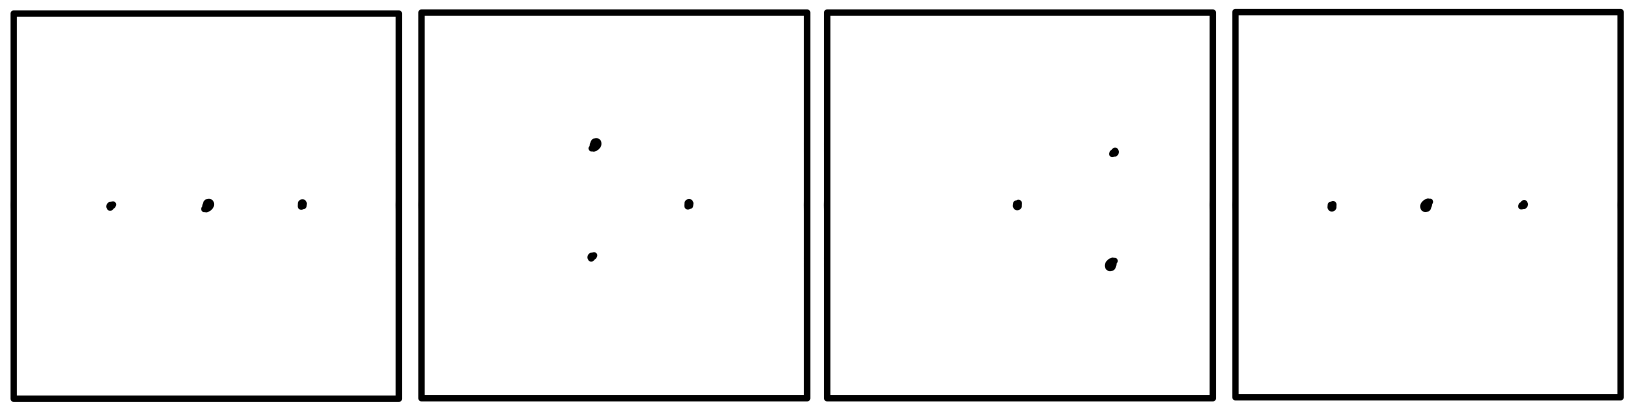
\includegraphics[width=0.8\textwidth]{classical_braids/1_classical_movie.png}
    \caption{Approximate frames of the movie of \cref{fig:classical_braid} at times \( t = 0, 1 / 3, 2 / 3, 1 \) (Left to Right)}
    \label{fig:classical_movie}
\end{figure}

Let \( M \) be the set of all possible movies of braids and therefore we will denote the map for the movie visualisation of the braid \( B \) as \( M : uB \to F \) where:
\[ M(B) = \{ F_t(B) \mid t \in [0, 1] \} \]

\begin{Remark}
For a given movie of a braid \( M(B) \), we can determine the image of the braid \( Im(B) \) by stacking braids on top of each other, and therefore determine the braid \( B \) modulo isotopy.
\end{Remark}

\subsection{Braid Diagrams and Crossings}

Let's consider instead a braid \( B \) and consider it's projection onto the \( xz \)-plane \( \text{proj}_{xz}(B) \) such that there are no points where multiple braids are crossing in the same instance or braids are intersecting in parallel, i.e. not more than 3 braids crossing simultaneously and no tangential points.
\[ \text{proj}_{xz}(B) = \{ (x, z) \in [0, 1]^2 \mid \exists t \in [0, 1] : (x, t, z) \in B\} \]
We want to encode the crossings onto the braid diagram and we therefore denote the set of all crossings, with position of intersections in \( [0, 1] \) and crossing type as \( C(B) \). 

Classical braids only admit two types of crossings, an overcrossing and an undercrossing. These are defined only in terms of an orientation.
We will arbitrarily define the orientation in the direction of projection, in this case the direction of the negative \( y \)-axis. 

Let \( Br \) be the set of all possible braid diagrams and let's denote the map for the braid diagram of the braid \( B \) as \( Br : uB \to Br \) where:
\[ Br(B) = (\text{proj}_{xy}(B), C(B)) \]

\begin{Remark}
    
Let's consider the braid diagrams as a graphical tool where we we denote overcrossings and undercrossings as

% Insert picture of overcrossing and undercrossing pictures
\begin{figure}[H]
    \centering
    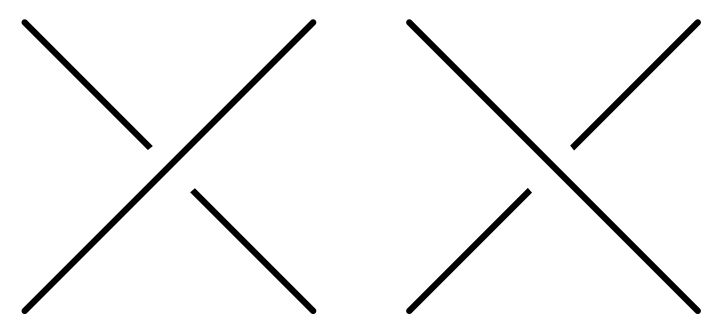
\includegraphics[width=0.40\textwidth]{classical_braids/2_classical_braid_crossings.png}
    \caption{Overcrossing (left) and Undercrossing (right)}
    \label{fig:overcrossing_undercrossing}
\end{figure}

Therefore the braid diagram of \cref{fig:classical_braid} would be

% Insert picture of braid described before. 
\begin{figure}[H]
    \centering
    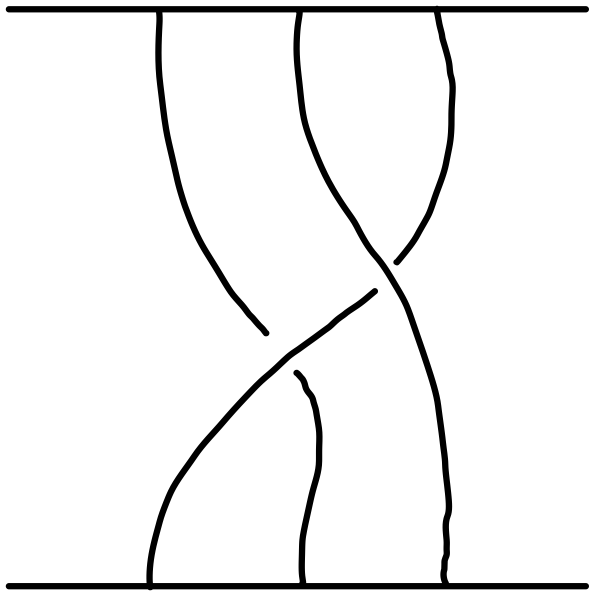
\includegraphics[width=0.25\textwidth]{classical_braids/3_classical_braid.png}
    \caption{Braid Diagram of \cref{fig:classical_braid}}
    \label{fig:classical_diagram}
\end{figure}
Noting that braid diagrams are modulo isotopy due to the braids themselves being considered under isotopy. 
\end{Remark}

\begin{Remark}
For a given braid diagram \( Br(B) \) we can determine the image of the braid \( B \) modulo isotopy by performing the inverse projection, this is possible because at the crossing points we know their relative order in the \( y \) direction, which is all the information we need modulo isotopy.  
\end{Remark}

\subsection{The Braid Group}

Let's consider the braids \( A, B \in uB_n \) and define a multiplication operation by considering stacking \( B \) on \( A \).
We can consider the \(x, y, \) and \( z \) components as \( A_x, A_y, \) and \( A_z \), similarly for \( B \), we therefore define. 
\[ 
AB := 
\begin{cases}
    (A_x(2t), A_y(2t), \frac{1}{2}A_z(2t)) &\text{for \( t \in [0, \frac{1}{2}]\)} \\
    (B_x(2t - 1), B_y(2t - 1) , \frac{1}{2}B_z(2t - 1) + \frac{1}{2}) &\text{for \( t \in (\frac{1}{2}, 1]\)} \\
\end{cases}
\]
Under stacking, braids form a group, where inverses is a flip along the xz plane or equivalently where \( t \mapsto 1 - t \), and the identity \( 1 \) is the braid without crossings. 

Let's consider a braid \( B \in uB_n \) and specifically it's braid diagram \( Br(B) \). 
We will then consider the sequence of crossings of the braid \( B \) where the order of the sequence is the order in which the crossings occur from the bottom to the top of the braid diagram, and the information of the index of the braids being crossed is recorded. 

Let's denote an overcrossing of strand \( i \) over strand \( i + 1 \) as \( \sigma_i \) and an undercrossing of strand \( i \) under strand \( i + 1 \) as \( \sigma_i^{-1} \). 
We can therefore denote any braid in \( uB_n \) as a sequence of crossings and convert the sequence of crossings equivalently as a concatenation of words \( \sigma_i \) and \( \sigma_i^{-1} \). 

Under our multiplication of the braid group we can define the multiplication of the words \( \sigma_i \) and \( \sigma_i^{-1} \) as concatenation, with the inverse of an overcrossing \( \sigma_i \) as an undercrossing \( \sigma_i^{-1} \) and the \( 1 \) as the identity. 

\begin{Example}
    Consider the braid diagram \cref{fig:classical_diagram}, this is described by \( \sigma_1 \sigma_2^{-1} \). 
\end{Example}

\begin{Example} \label{ex:stacking}
Consider the following stacking operation in \( uB_3 \), where \( A = \sigma_1 \sigma_2 \) and \( B = \sigma_1 \sigma_2^{-1} \). 
We compute \( AB = \sigma_1\sigma_2\sigma_1\sigma_2^{-1} \) by stacking the braid diagrams on top of each other. 

% Insert picture of braid
\begin{figure}[H]
    \centering
    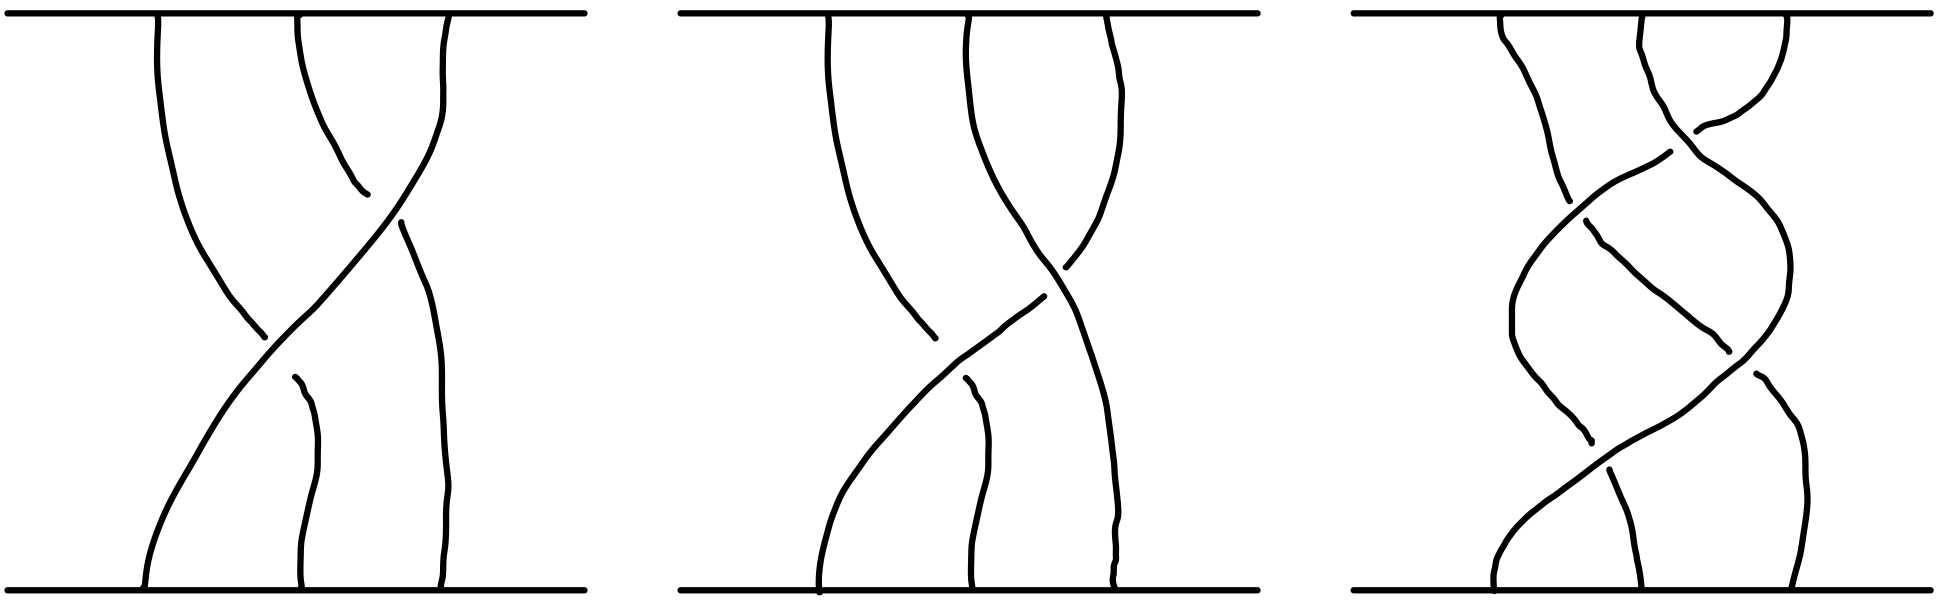
\includegraphics[width=0.8\textwidth]{classical_braids/4_classical_braid_stacking.png}
    \caption{\( A \) (Left), \( B \) (Centre), \( AB \) (Right)}
\end{figure}

\end{Example}

\begin{Definition}[The Artin Relations for Braids]
The relations defined on the braid group are the Artin Relations
\begin{alignat*}{3}
    \sigma_i\sigma_{i + 1}\sigma_i &= \sigma_{i + 1}\sigma_i\sigma_{i + 1} \\
    \sigma_i \sigma_i^{-1} &= \sigma_i^{-1} \sigma_i = 1 \\
    \sigma_i\sigma_j &= \sigma_j \sigma_i &&\text{ where \( |i - j| > 1\)}
\end{alignat*}
\end{Definition}

\begin{Exercise}
    Explain why \( \mathit{uB}_2 \) is isomorphic to \( \Z \).
\end{Exercise}
\begin{Exercise}
    Prove \( \sigma_1^{-1} \sigma_2 \sigma_1 = \sigma_2 \sigma_1 \sigma_2^{-1} \) in \( \mathit{uB}_3 \), verify this using a braid diagram.
\end{Exercise}

\section{Operadic Composition for Classical Braids}

% Fix this in the morning!

We want to define \( A \circ_i B \) for braids \( A \in uB_n \) and \( B \in uB_m \) and strand index \( i \in [n] \). 
We're going to do this by considering the braid diagram of \( A \) and consider a small region around the \( i \)th strand, and then replacing this region with the braid diagram \( B \).

There are alternate ways of defining this operation.
Specifically, we could consider a region around the \( i \)th strand of \( A \) and this with \( B \) at each height, however, the definition we will give generalises to welded braids, and infact is the more intuitive definition of composition of braids. 

Consider the  braid diagrams \( Br(A) \) and \( Br(B) \).
% Let the number of crossings of a braid \( A \) be denoted \( k_A \) and let's arbitrarily choose a representative braid for \( A \) and \( B \) such that a crossing occurs on the braid diagram at linearly spaced intervals vertically on the braid diagram. 
% I.e. a crossing occurs at the heights \( \{ \frac{i}{k_A + 1} \in [0, 1] \mid i \in [k_A] \} \).
% Let's first assume that \( k_A \) and \( k_b \) are coprime, so that crossings occur at different heights of \( Br(A) \) and \( Br(B) \). 
We're going to define the notation \( Br_i(A) \) to be the braid diagram of the \( i \)th strand of \( A \). 

Consider \( Br_i(A) \) translated in the positive \( x \) direction by \( r \), call this \( Br_i^r(A) \). 
Let \( \varepsilon > 0 \) be such that both curves \( Br_i^{\pm\varepsilon}(A) \) are equivalent under isotopy to \( Br_i(A) \). 
We know this exists as if it were not to exist, then with a small perturbation of \( Br_i(A) \) in \( x \) will cause a extra crossing to occur or for a crossing not to occur, which can occur only if the curve \( Br_i(A) \) was tangent to another braid, which is not possible for any braid diagram. 

\begin{figure}[H]
    \centering
    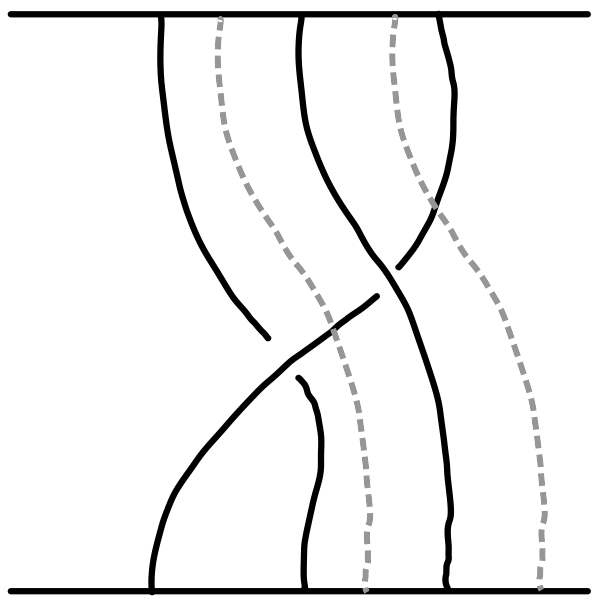
\includegraphics[width=0.4\textwidth]{images/classical_braids/5_classical_braid_composition_region.png}
    \caption{\( Br_3^{\pm\varepsilon}(A) \) (grey dashed) for \( A = \sigma_1 \sigma_2^{-1} \in uB_3 \)}
    \label{fig:classical_composition_region}
\end{figure}

Let's now consider the region enclosed by the curves \( Br_i^{\pm\varepsilon}(A) \), call this \( R_i^{\varepsilon}(A) \). 
We then consider for all heights \( t \in [0, 1] \), replacing the slice of the region \( R_i^\varepsilon(A) \) at that height with the slice of the horizontal height of \( Br(B) \). 

We now want to consider the crossings after this replacement.
We can distinguish two types of crossings on the inputted braid \( B \), the crossings formed by the the strands of \( B \) with themselves, and the crossings formed by the strands of \( B \) with \( A \)
The crossings of the former aren't effected, however the crossings of the latter are defined by the order in which the the crossings of \( Br_i(A) \) occurred from top to bottom. 
We're guaranteed this is possible, because we know that since \( Br_i^{\pm\varepsilon}(A) \) are both equivalent to \( Br_i(A) \), then anything in between them must be. 

\begin{figure}[H]
    \centering
    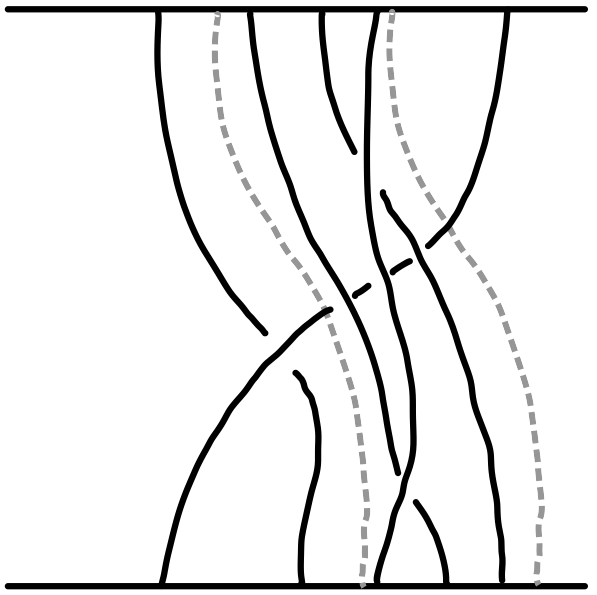
\includegraphics[width=0.4\textwidth]{images/classical_braids/6_classical_braid_composition.png}
    \caption{\( A \circ_3 B \), where \( A \) and \( B \) are defined in \cref{ex:stacking}.}
    \label{fig:classical_composition}
\end{figure}

Finally we can deform the current braid-like object to be linearly spaced along the top and the bottom of the diagram. 

Our definition is flawed however.
If the two braids are both under isotopy, the order in which the crossings occur could be different under the composition of different representatives. 
Let's decide to choose a representative \( A \) where crossings occur linearly spaced along the height of the braid. 
\begin{Example}
For the braid \( \sigma_1 \sigma_2 \in uB_3 \), there will be two crossings at the heights \( t = \frac{1}{3} \) and \( t = \frac{2}{3} \) under this specification. 
\end{Example}
The issue with our composition operation occurs when two crossings occur simultaneously at the same height. 
If this occurs, then we arbitrarily decide on the order in which the crossings occur. 
This is justified, as any decision would be equivalent modulo isotopy. 

\begin{Example}
    Consider \( A = \sigma_1 \in uB_2 \) and \( B = \sigma_2^{-1} \in uB_3 \), \( A \circ_2 B \) is computed diagrammatically as

    % Picture of the composition of braids. 
    \begin{figure}[H]
    \centering
    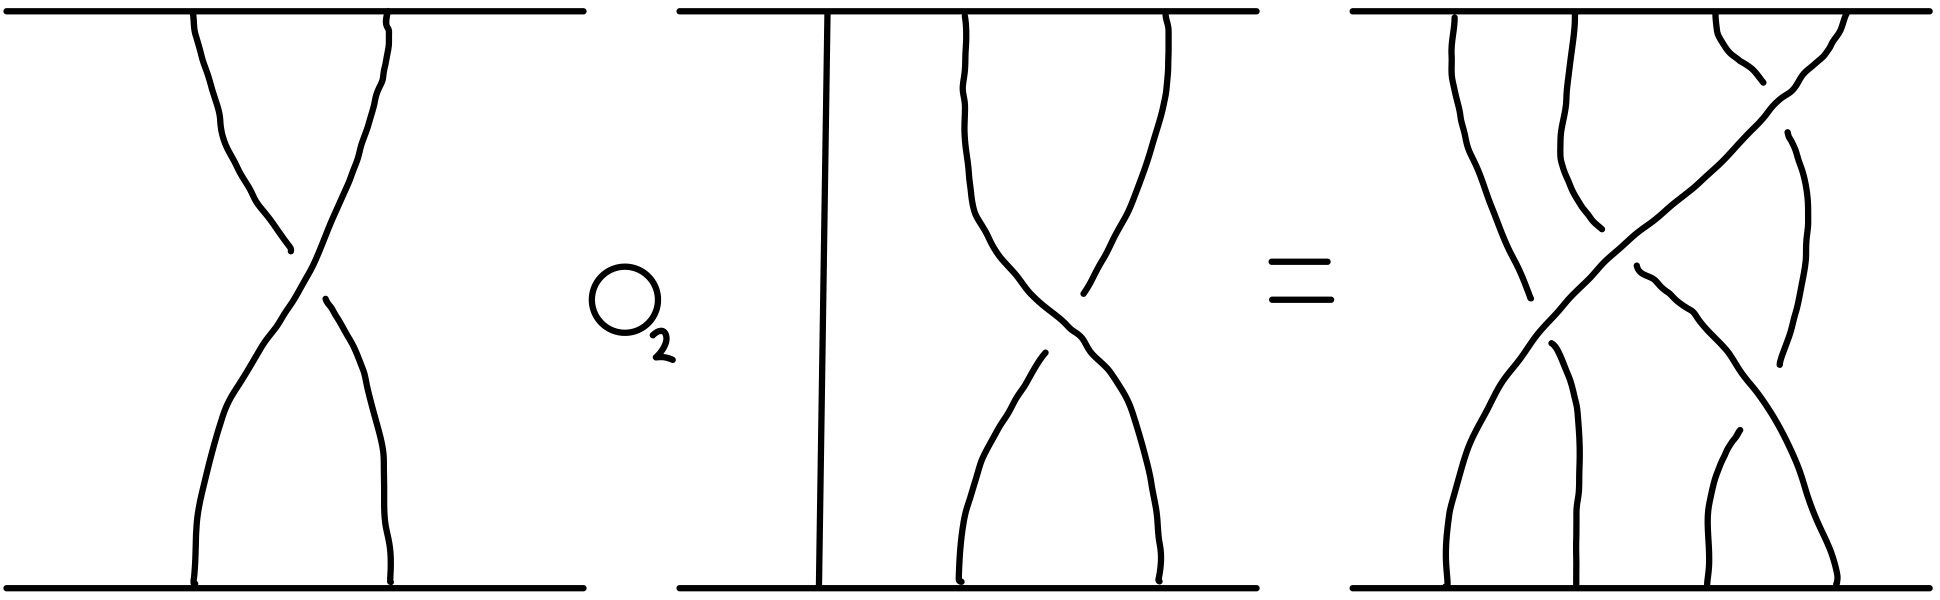
\includegraphics[width=0.8\textwidth]{classical_braids/7_classical_braid_composition_example.png}
    \caption{Composition of \( B \) (middle) into the \( 2 \)nd strand of \( A \) (left) which computes \( A \circ_2 B \) (right).}
\end{figure}

    Therefore getting the braid \( A \circ_2 B = \sigma_3^{-1} \sigma_1 \sigma_2 \sigma_3 \in uB_4 \). 
\end{Example}

\begin{Exercise}
    Determine the braid diagram for \( A = \sigma_1 \sigma_2 \in uB_3 \), \( B = \sigma_2^{-1} \), and \( A \circ_2 B \). 
\end{Exercise}
\begin{Exercise}
    Let \( A = \sigma_2 \sigma_3 \sigma_1^{-1} \sigma_3 \in uB_4 \) and \( B = \sigma_1^3 \in uB_3 \). 
    Using braid diagrams, compute: \( A \circ_2 B \), \( B \circ_1 A \), \( A \circ_2 1 \) where \( 1 \in uB_2 \), and \( 1 \circ_2 B \) where \( 1 \in uB_5 \).
\end{Exercise}
\begin{Exercise}
    Show that classical braids form a canonical operad structure under this composition we described.
\end{Exercise}